\documentclass[12pt]{report}

%Vous souciez pas de tout les packages, j'ai oublié ce que fait la moitié d'entre eux

\usepackage[utf8]{inputenc}
\usepackage[T1]{fontenc}
\usepackage[francais]{babel}
%\usepackage{layout}
\usepackage[left=3cm,right=3cm,top=3cm,bottom=3cm]{geometry}
%\usepackage{setspace}
\usepackage{soul}
\usepackage[normalem]{ulem}
%\usepackage{eurosym}
%\usepackage{bookman}
%\usepackage{charter}
%\usepackage{newcent}
%\usepackage{lmodern}
%\usepackage{mathpazo}
%\usepackage{mathptmx}
%\usepackage{url}
%\usepackage{verbatim}
%\usepackage{moreverb}
%\usepackage{listings}
%\usepackage{fancyhdr}
%\usepackage{wrapfig}
\usepackage{color}
%\usepackage{colortbl}
\usepackage{amsmath}
\usepackage{amssymb}
\usepackage{mathrsfs}
%\usepackage{asmthm}
%\usepackage{makeidx}
\usepackage{graphicx}
\usepackage{tabularx}
\usepackage{tgtermes}
\usepackage{titlesec}
\usepackage[final]{pdfpages} 
\usepackage{epsfig}
\usepackage{comment}
\usepackage{float}
\usepackage{amsmath}
\renewcommand{\emph}{\textit}
\renewcommand{\thesection}{\arabic{section}}
\renewcommand{\thesubsection}{\arabic{section}.\arabic{subsection}}
\titleformat*{\subsection}{\bfseries}
\parskip=5pt

%Information pour la page de garde

\title{TP2 - Reconstruction 3D}
\author{Jean-Baptiste \bsc{Morice}, Guillaume \bsc{Versal}}
\date{\today}

\begin{document}

%Commande qui crée la page de garde
\maketitle

\tableofcontents

\newpage
\section*{Introduction}

Ce TP à pour objectif de nous faire calculer une carte de disparité entre deux images selon différents critères tel que le " Winner takes all" ou encore le SSD,"Sum of Squared Differences". La carte de disparité est un outil permettant de voir l'information sur les correspondances des points entre deux images d'une même séances avec des points de vue différent.

\section{Notre travail}

\subsection*{Question 1}

Dans un premier temps, nous devions vérifier qualitativement que les images sont bien rectifiées. Pour ce faire, on regarde dans les différentes images certain points particulier dans les deux images et si ces derniers ne sont pas au même niveau dans les deux images alors, les images ne sont pas rectifiée.

\begin{figure}
\begin{center}
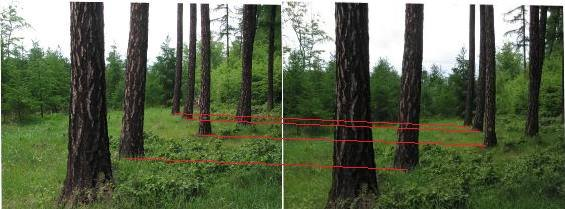
\includegraphics[scale=0.7]{Images/cedar.jpg} 
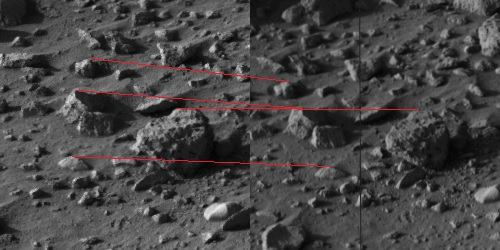
\includegraphics[scale=0.8]{Images/rocher.jpg} \\
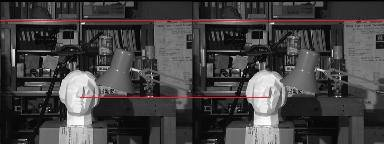
\includegraphics[scale=1]{Images/tsukuba.jpg} 
\caption{Comparaison de point d'intérêt}
\end{center}
\end{figure}

Comme on peut l'observer sur les images comparatives, la seule paire d'image qui vérifie ce critère c'est \texttt{tsukuba-r.pgm} et \texttt{tsubuka-l.pgm}. Cela se remarque notamment très bien au niveau des étagères présentes dans le fond de l'images. Concernant les autres images, on observe très nettement sur l'image des rochers que ces derniers ne sont pas au même niveau, il en va de même pour les images \texttt{cedar}, même si c'est un peu moins visible.

\subsection*{Question 2, 3 et 4}

Dans la suite de ce TP, nous devions réaliser la carte de disparité des images \texttt{tsukuba}. Nous devions réaliser deux méthodes et comparer ces dernières. Dans un premier temps, nous avons implémenté la méthode nommée \textit{"Winner takes all"}. Avec cette méthode, on obtient le résultat présent en figure 2.

Dans un second temps, nous avons implémenter la méthode nommée \textit{"Sum of Squared Differences"}. Contrairement à la méthode précédente, cette fois-ci on réalise les calculs sur une fenêtre, le tout régulé par un noyau. Avec cette méthode, nous obtenons les résultats suivants.

Nous pouvons constaté que la SSD obtient un meilleur résultat. Cela est du au faite qu'avec la SSD, nous prenons en compte non pas un pixel mais une fenêtre ce qui nous permet d'avoir un résultat beaucoup plus précis. De plus, plus la taille de cette fenêtre est importante, plus le résultat est bon. Malgré tout, avec l'augmentation de la taille de la fenêtre, le temps de calcul devient plus important et  cela peut-être handicapant pour certaine utilisation.

\section{Conclusion}
 
 Ce TP nous a permis de nous familiariser avec les cartes de disparité, aussi bien au niveau de leur réalisation que de leur interprétation. 

\begin{comment}

%Commande pour le sommaire

\renewcommand{\contentsname}{\large Sommaire} % Change le nom en sommaire
\setcounter{tocdepth}{2} % Défini la profondeur d'une table des matières
\tableofcontents
\newpage

\end{comment}

\newpage


%Commande pour le sommaire des figures

\renewcommand*\listfigurename{\large Liste des figures}
\listoffigures
\newpage


\end{document}
